\documentclass{article}
\usepackage{graphicx}
\usepackage{amsmath}
\usepackage{hyperref}
\usepackage{listings}
\usepackage{xcolor}

% styling for listings
\lstset{
  basicstyle=\ttfamily\small,
  keywordstyle=\color{blue}\bfseries,
  commentstyle=\color{gray}\itshape,
  stringstyle=\color{orange},
  breaklines=true,
  frame=single,
  numbers=left,
  numberstyle=\tiny\color{gray},
  captionpos=b,
}

\title{Diabetes Classifier: A Classifier using Grammatical Evolution on a Reduced Diabetes Dataset}
\author{Hoang Tu Bui - 24005665}
\date{\today}

\begin{document}

\maketitle

\begin{abstract}
    This project explores the use of Grammatical Evolution (GE) to develop a classification model for predicting diabetes using a reduced dataset.
    The objective is to evaluate the effectiveness of evolving classification programs through GE to improve understanding of evolutionary algorithms in classification tasks.
    The algorithm use mean squared error as the main fitness function to evaluate the programs and number of unique features used in the program as a secondary fitness function to encourage the model to use more features.
    The model achieved an accuracy of 0.7467 on the training data and 0.6985 on the test data, with a mean squared error (MSE) of 0.1677 on the training data.

\end{abstract}


\section{Problem Statement}
This study explores the application of Grammatical Evolution as a classification technique for predicting diabetes using the reduced-size version of the Diabetes dataset.
The dataset consists of 21 features, including 7 numerical and 14 boolean features. The training set includes 5,042 samples, while the test set contains 95,804 samples.
The project aims to evaluate the effectiveness of evolving classification programs through GE contributing to both the understanding of evolutionary algorithms in classification tasks.


\section{Data Preprocessing}
After features exploration, it is clear that the dataset contains 21 features, including 7 numerical features, 14 boolean features and no categorical features in the dataset.
The training data don't have any missing values, so there is no need to handle missing values in this dataset.
That leaves us with the task of normalizing the numerical features.

Out of the 7 numerical features, 2 of them (Age and BMI) are continuous and the rest are discrete. 
Plotting the histograms of the continuous features, we can see that both of them are normally distributed.
Thus, standard scaling is applied to normalize them.
Figure \ref{fig:histograms} shows the histograms of the continuous features.

\begin{figure}[h]
    \centering
    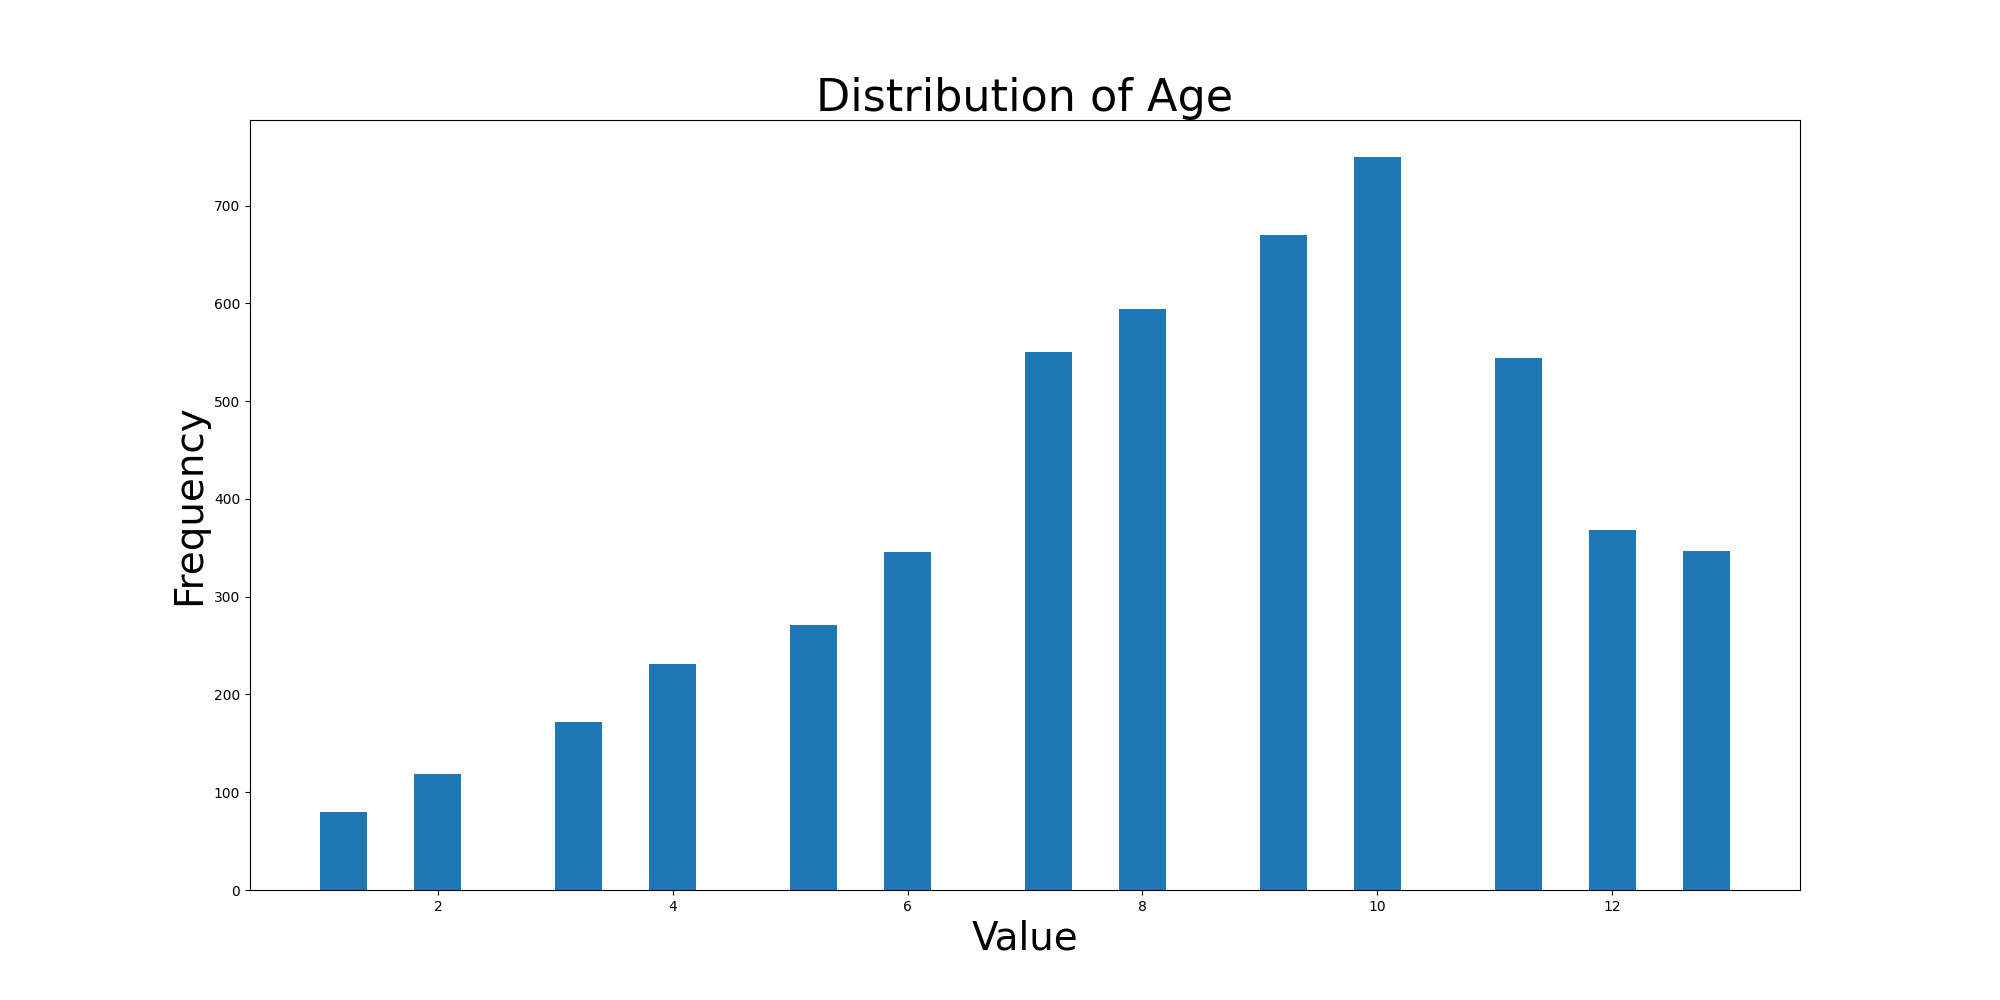
\includegraphics[width=0.8\textwidth]{./figures/hist-Age.png}
    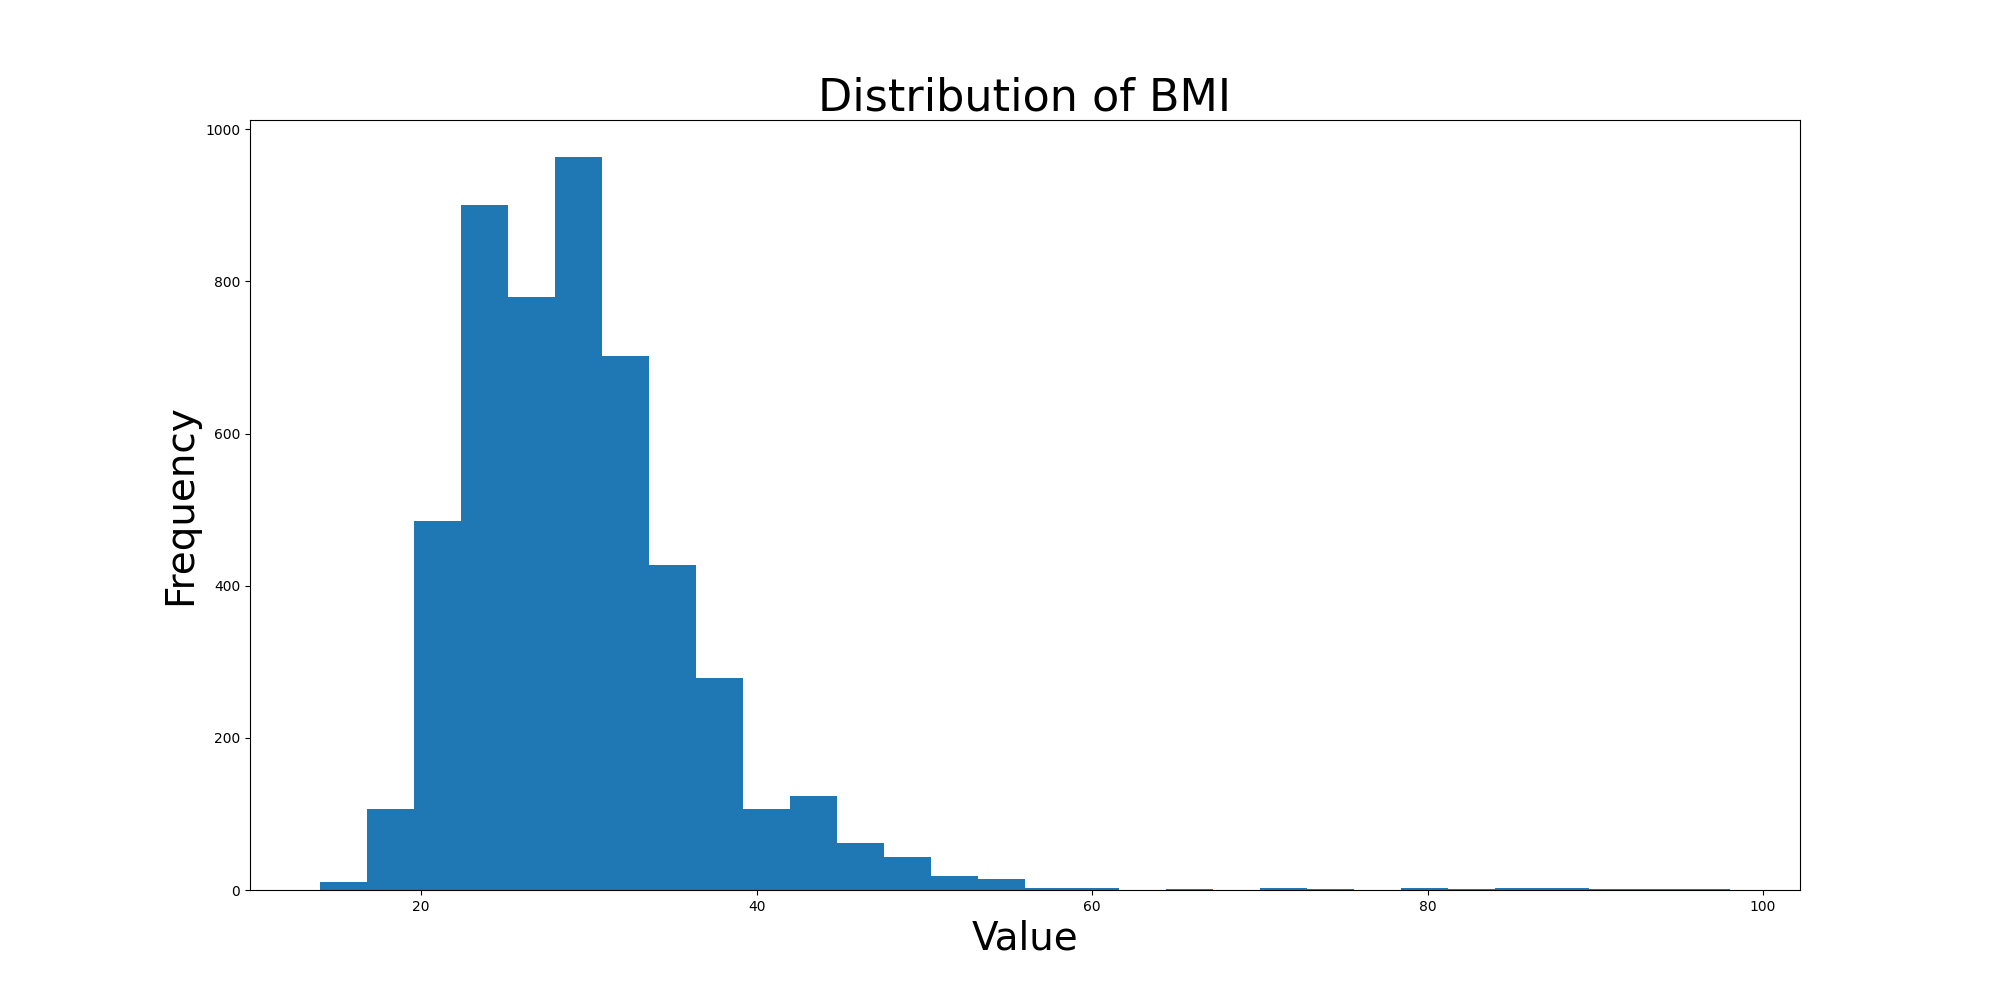
\includegraphics[width=0.8\textwidth]{./figures/hist-BMI.png}
    \caption{Histograms of the continuous features (Age and BMI)}
    \label{fig:histograms}
\end{figure}

\begin{figure}[h]
    \centering
    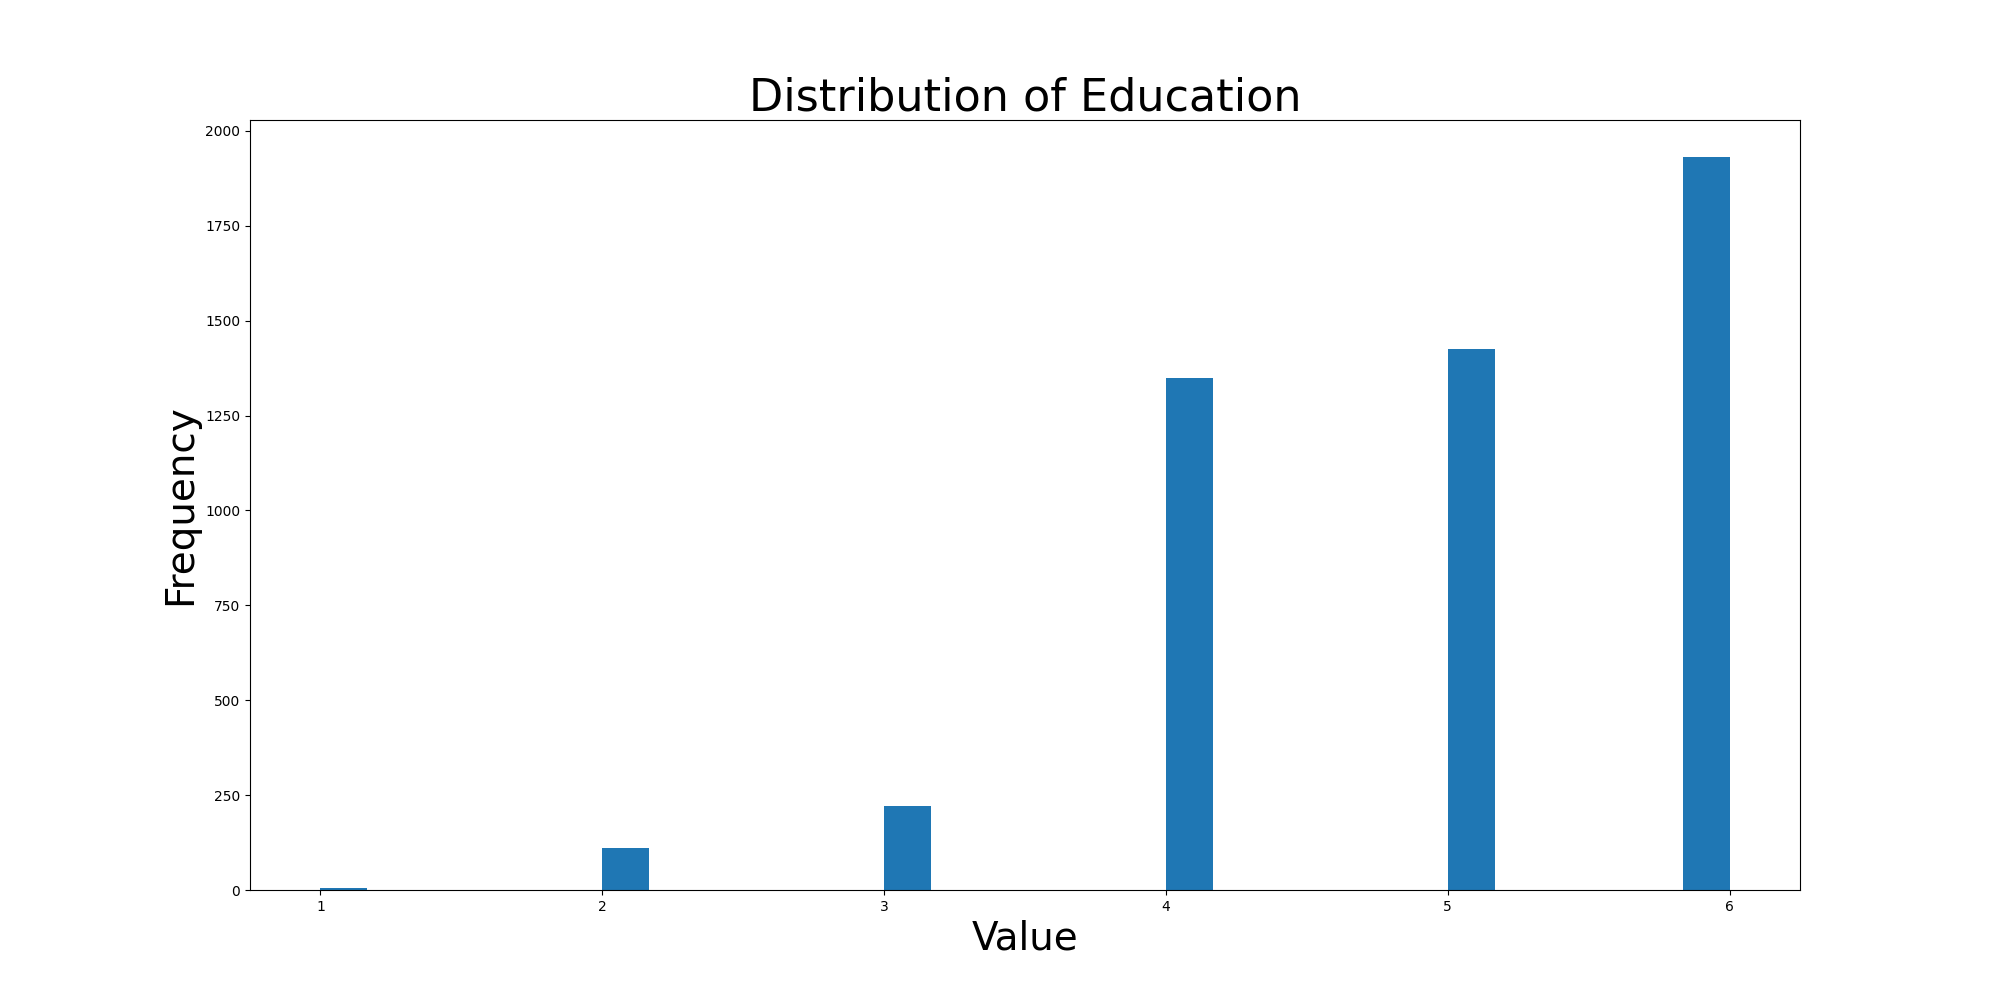
\includegraphics[width=0.8\textwidth]{./figures/hist-Education.png}
    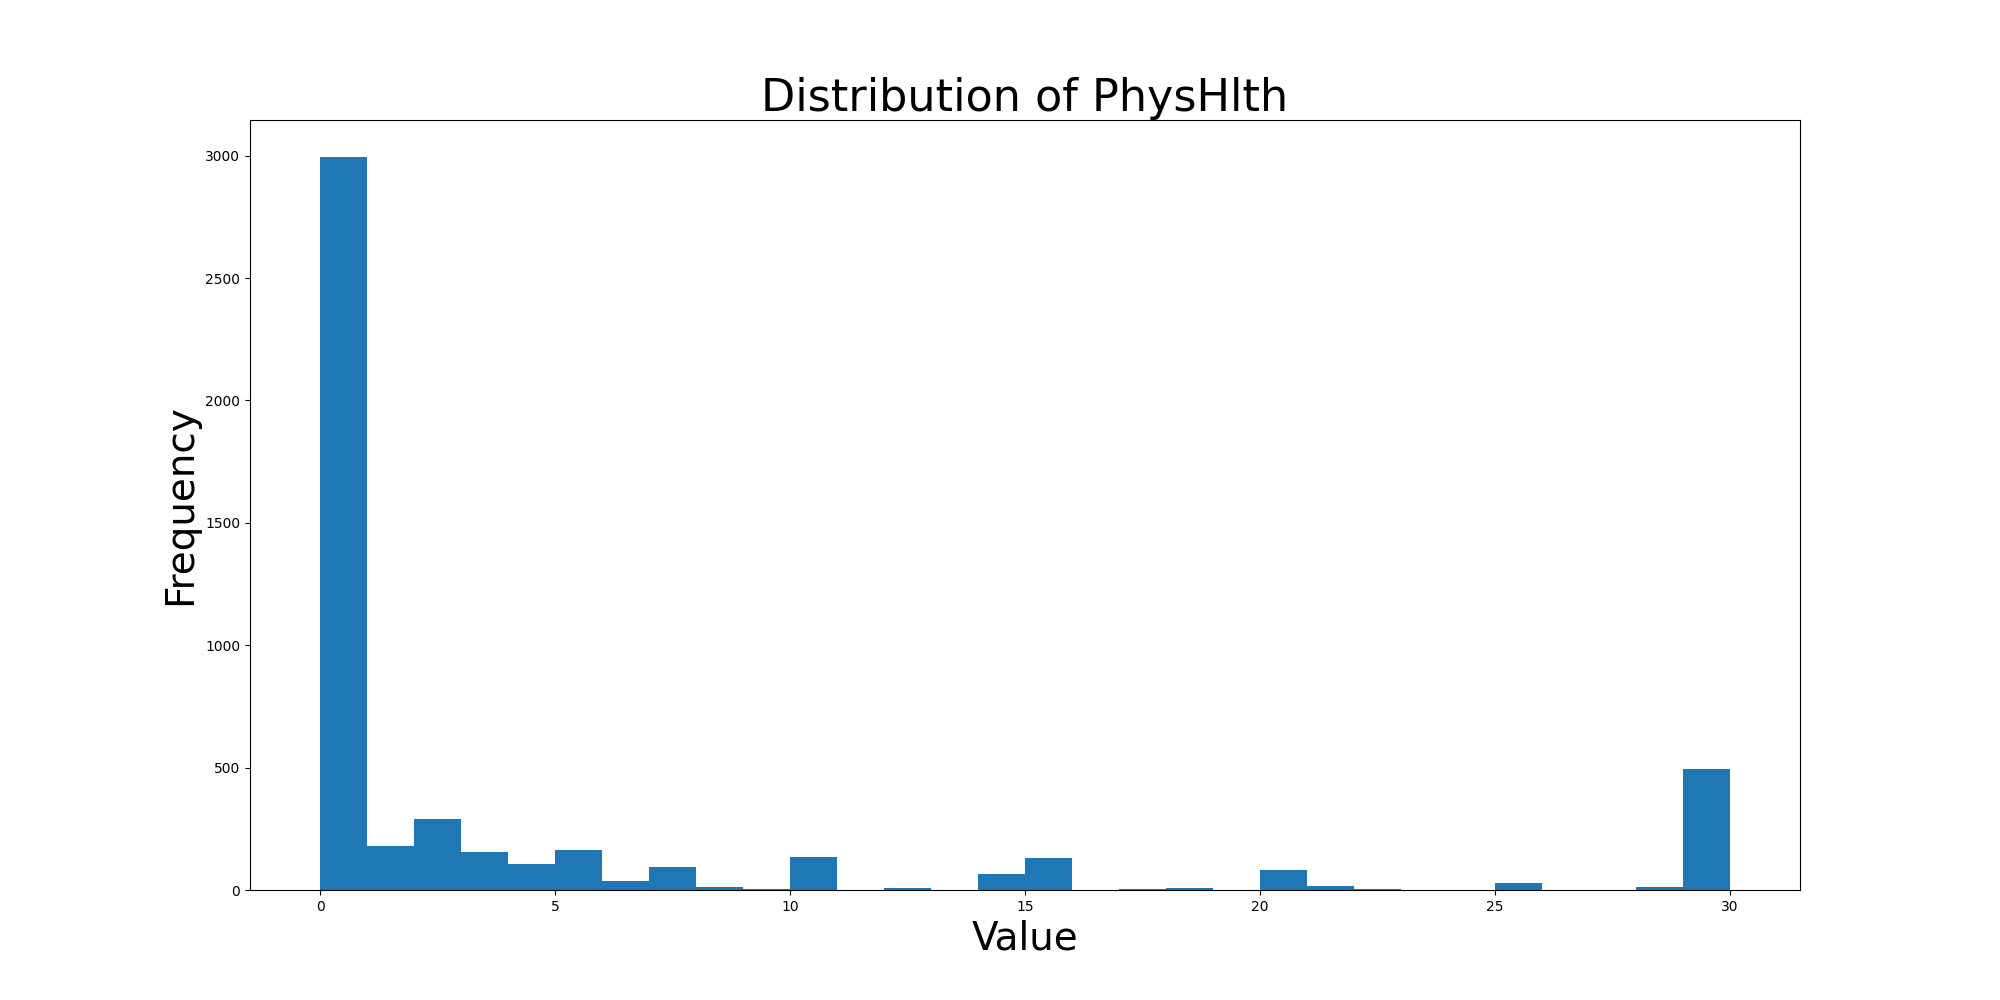
\includegraphics[width=0.8\textwidth]{./figures/hist-PhysHlth.png}
    \caption{Histograms of the discrete features (Education and Physical Health)}
    \label{fig:histograms-discrete}
\end{figure}

While normally the discrete features would be leave as they are but some of them have up to 30 unique values (MentHlth, PhysHlth), which could lead to bias in the model so I decided to apply min-max scaling to them.
Standard scaler is not used in this case because the data distribution is not normal, using it could distort the meaning of the data.
The histograms of the discrete features are shown in Figure \ref{fig:histograms-discrete}.


\section{Model Selection and Training}
The model is trained using the Grammatical Evolution algorithm.
GE is a genetic programming technique that generates solutions to problems by evolving computer programs. 
It uses a BNF (Backus-Naur Form) grammar to define the structure of valid solutions.
In this section, I will explain the grammar used to generate the classification programs, the fitness function used to evaluate the programs, and the training process.

    \subsection{Grammar}
    The grammar used to generate the classification programs is defined as follows:

    \begin{verbatim}
        <number_op> ::= 
            add(<number_value>, <number_value>)
            | sub(<number_value>, <number_value>)
            | mul(<number_value>, <number_value>)
            | div(<number_value>, <number_value>) 
            | abs(<number_value>)
            | sigmoid(<number_value>)
            | tanh(<number_value>)
            | relu(<number_value>)
            | swish(<number_value>)
            | np.where((<logic_op>), (<number_value>), (<number_value>))

        <logic_op> ::= 
            <compare_op>
            | and_(<logic_op>, <logic_op>)
            | or_(<logic_op>, <logic_op>)
            | xor(<logic_op>, <logic_op>)
            | not_(<logic_op>)
            | <bool_feat>

        <compare_op> ::=
            greater_than(<number_value>, <number_value>)
            | less_than(<number_value>, <number_value>)
            | in_range(<number_value>, <number_value>, <number_value>)

        <number_value> ::=
            <number_op>
            | <number_feat>
            | <number>
            | <logic_op>

        <number> ::= 
            <d>.<d><d><d><d>
            | -<d>.<d><d><d><d>

        <d> ::= 0 | 1 | 2 | 3 | 4 | 5 | 6 | 7 | 8 | 9



        <number_feat> ::= 
            nf[0]
            | nf[1]
            | nf[2]
            | nf[3]
            | nf[4]
            | nf[5]
            | nf[6]
        <bool_feat> ::= 
            bf[0]
            | bf[1]
            | bf[2]
            | bf[3]
            | bf[4]
            | bf[5]
            | bf[6]
            | bf[7]
            | bf[8]
            | bf[9]
            | bf[10]
            | bf[11]
            | bf[12]
            | bf[13]
    \end{verbatim}

    This grammar defines various types of expressions and operations that can be used in the generated classification programs. The key components are as follows:

    \begin{itemize} 
        \item \textbf{number\_op}: Operations that return a numerical value, such as arithmetic operations (add, sub, mul, div), mathematical functions (abs, sigmoid, tanh, relu, swish), and conditional expressions (np.where). 
        \item \textbf{logical\_op}: Operations that return a boolean value, including comparisons (greater\_than, less\_than, in\_range) and logical operations (and\_, or\_, xor, not\_). 
        \item \textbf{compare\_op}: Operations used to compare two numbers, such as checking for greater than, less than, or within a range. 
        \item \textbf{number\_value}: Any expression that evaluates to a number, which can be a number, a numerical feature, or the result of an operation. 
        \item \textbf{number}: Literal numbers, specified in the range from $-9.999$ to $9.999$, expressed using digits. 
        \item \textbf{d}: A digit from 0 to 9, used to form literal numbers. 
        \item \textbf{number\_feat}: Numerical features derived from the dataset, such as feature values nf[0], nf[1], etc. 
        \item \textbf{bool\_feat}: Boolean features from the dataset, represented as bf[0] through bf[13]
    \end{itemize}

    The grammar is designed to allow the generation of classification programs that can combine numerical and boolean features, perform arithmetic and logical operations, and make decisions based on conditions. 
    The programs generated using this grammar can be used to classify the diabetes dataset based on the input features.
    Upon running the generated programs on the dataset, the programs will output a numerical value that is then fed into a sigmoid function to obtain the classification probability.
    Which is then used to classify the data into 0 or 1 based on a threshold of 0.5.
    
    Instead of using \textbf{logic\_op} as the root of the program, I decided to use \textbf{number\_op} as the root of the program.
    This approach allows more flexibility in choosing the fitness function and the way the program is evaluated.

    Another detail worth mentioning in this grammar is \textbf{logic\_op} can be used as a \textbf{number\_value} in \textbf{number\_op}. 
    This allows more complex combinations of logical and numerical operations in the generated programs.
    Since the root of the program is \textbf{number\_op}, \textbf{bool\_feat} has very limited usage if not being considered a numerical value.


    \subsection{Fitness Function}
    Given the model described above, which outputs the probability of a data point being classified as positive for diabetes, we have several options for defining the fitness function, including accuracy, log-loss, and mean squared error.
    However, it is clear that mean squared error (MSE) and log-loss are more informative choices than accuracy, as they provides a more granular view of the model's performance by penalizing large deviations between predicted probabilities and actual outcomes. 
    After conducting some experiments and evaluating the performance of different fitness functions, I decided to use MSE as the final choice for the fitness function.

    In addition to the mean squared error, I also added a second objective for the programs that use more features.
    This fitness function is defined as sigmoid of number of unique features used in the program.
    This is to encourage the model to use more features in the classification process, as using more features can potentially lead to better classification performance.
    The sigmoid function is used to moderately promote using more features when the model is only using a small number of them but still leave room for feature selection.
    The reward helps leading the population to the right direction during the first few generations, when the programs are still random and have not yet learned the dataset.


    \subsection{Training Process}
    \label{subsec:training-process}

    After preprocessing the data and defining the grammar and fitness function, the next step is to train the model using the Grammatical Evolution algorithm.
    Similar to other genetic algorithms, the GE algorithm involves the following steps:
    \begin{enumerate}
        \item \textbf{Initialization}: Create an initial population of random programs based on the grammar. 
        \item \textbf{Mapping}: Map the individuals to the program using the grammar.
        \item \textbf{Evaluation}: Execute the programs on the training data and evaluate the fitness of each program using the fitness function. 
        \item \textbf{Selection}: Select the best individuals based on the fitness score. 
        \item \textbf{Evolution}: Evolve the population through genetic operations crossover and mutation.
    \end{enumerate}
    Since the grammar has different treatment for numerical and boolean features, the features are split into numerical and boolean features (nf and bf) to match the grammar defined above.

    One of the key challenges in the training process is that the evolutionary algorithm often produces individuals that map to the same program, making it difficult to achieve meaningful improvements in later generations. To address this issue, I implemented two strategies:
    \begin{itemize}
        \item \textbf{New Individual Comparator}: In hall of fame, I used a comparator that compares the phenotypes of the individuals instead of the individuals themselves. This ensures that only unique programs are retained. However, this approach somehow limits the convergence rate of the population making the evolution process significantly slower so it is not used in the final model.
        \item \textbf{Periodic Deduplication}: After a certain number of generations, filter the hall of fame to remove duplicates. This periodic deduplication encourages diversity and mitigates stagnation in the evolutionary process.
    \end{itemize}

    The parameters used in the training process are as follows:
    \begin{lstlisting}[language=Python, caption={Configuration Parameters for Evolutionary Algorithm}, label={lst:config}]
        POPULATION_SIZE = 1000
        MAX_GENERATIONS = 200
        FILTER_INTERVAL = 100
        P_CROSSOVER = 0.8
        P_MUTATION = 0.01
        HALLOFFAME_SIZE = max(round(0.01 * POPULATION_SIZE), 1)  # it should be at least 1
        ELITE_SIZE = min(round(0.01 * POPULATION_SIZE), HALLOFFAME_SIZE)
        
        CODON_CONSUMPTION = "lazy"
        GENOME_REPRESENTATION = "list"
        MAX_GENOME_LENGTH = None
        
        MAX_INIT_TREE_DEPTH = 17
        MIN_INIT_TREE_DEPTH = 5
        MAX_TREE_DEPTH = 90
        MAX_WRAPS = 0
        CODON_SIZE = 255
    \end{lstlisting}
    Experimenting with different values for the interval, I found that the best results were achieved when the hall of fame was filtered every 100 generations.
    Changing the population size, crossover rate, mutation rate, and other parameters did not significantly improve the performance of the model, so the default values were used.
        

\section{Evaluation and Results}
This section presents the evaluation results of the evolutionary model on the training and test datasets, with accuracy as the primary performance metric.

After training the model for 200 generations with the setup described in Section \ref{subsec:training-process}, the best program found by the evolutionary algorithm achieved an accuracy of 0.7467 on the training data and 0.6985 on the test data. The model utilizes 21 features and achieved a mean squared error (MSE) of 0.1677 on the training data.
The best program found by the evolutionary algorithm is:
\begin{lstlisting}[language=Python, caption={Best Program Found by the Evolutionary Algorithm}, label={lst:best-program}]
    mul(sub(nf[2], sub(xor(not_(bf[13]), xor(greater_than(bf[2], not_(bf[1])), xor(not_(or_(bf[5], xor(bf[4], not_(in_range(nf[1], bf[2], sub(xor(not_(bf[13]), xor(bf[10], bf[13])), sub(nf[2], sub(sub(abs(nf[1]), sub(nf[2], -0.9059)), not_(or_(bf[5], or_(bf[5], xor(bf[4], bf[0])))))))))))), bf[13]))), sub(nf[2], sub(xor(not_(bf[13]), xor(bf[0], bf[13])), sub(nf[2], sub(sub(abs(swish(nf[1])), sub(nf[2], swish(sub(1.8002, nf[0])))), nf[1])))))), sigmoid(swish(nf[6])))
\end{lstlisting}


To better understand the model's performance across generations, I tracked the error rate (mean squared error) and number of features used for each generation during training. 
Figure \ref{fig:error-rate-plot} and Figure \ref{fig:feature-plot} show the progression of the error rate and number of features used over the course of the training process.
\begin{figure}[h] 
    \centering 
    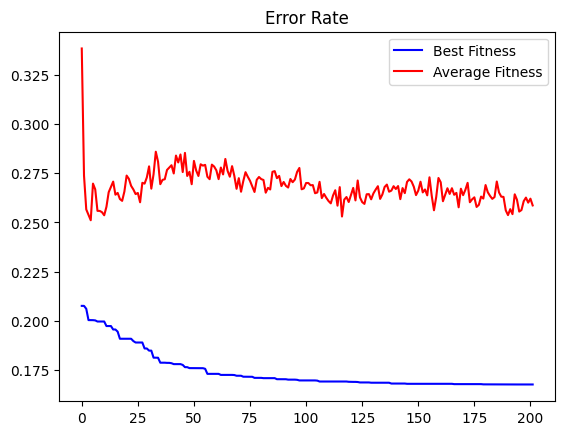
\includegraphics[width=0.8\textwidth]{./figures/error-rate-plot.png} 
    \caption{Error Rate Plot} 
    \label{fig:error-rate-plot}
\end{figure}
\begin{figure}[h] 
    \centering 
    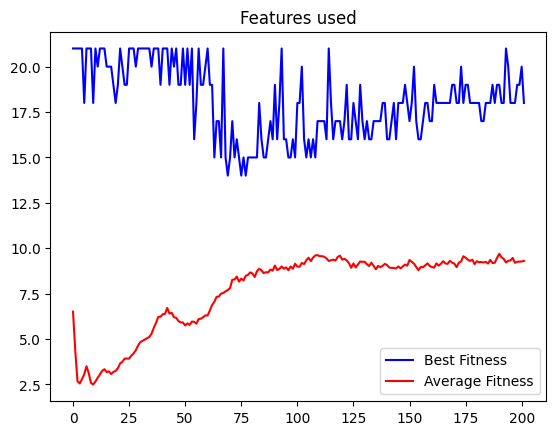
\includegraphics[width=0.8\textwidth]{./figures/feature-used-plot.png} 
    \caption{Number of Features Used Plot} 
    \label{fig:feature-plot}
\end{figure}
It can be seen that the average number of features used in the programs increases over time, indicating that the model is learning to utilize more features for classification.

In addition to the error rate plot, the confusion matrix of the best program is shown in Figure \ref{fig:confusion-matrix}. This matrix provides insights into the model's classification performance, showing the distribution of predictions across the four categories: True Positives (TP), True Negatives (TN), False Positives (FP), and False Negatives (FN).
\begin{figure}[h] 
    \centering 
    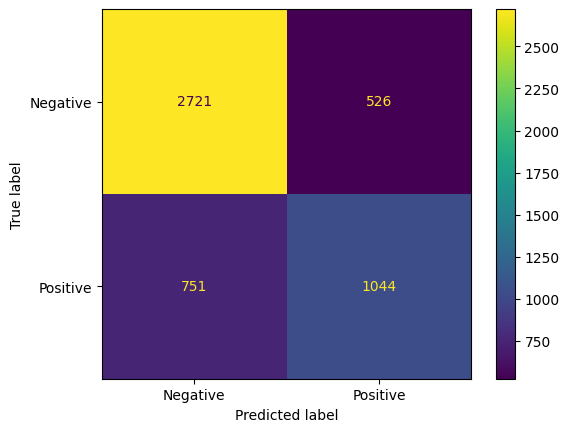
\includegraphics[width=0.8\textwidth]{./figures/confusion-matrix.png} 
    \caption{Confusion Matrix of the Best Program} 
    \label{fig:confusion-matrix}
\end{figure}



\section{Conclusion}
This study explored the application of Grammatical Evolution as a classification technique for predicting diabetes using the reduced-size version of the Diabetes dataset.
The model achieved an accuracy of 0.7467 on the training data and 0.6985 on the test data, with a mean squared error (MSE) of 0.1677 on the training data.
Mean squared error of 0.1677 on the training data indicates that there is still room for improvement in the model's performance.
There are still improvement in the last 10 generations of the model, so it is possible to achieve better results with more training generations.

In addition, binary cross entropy should be considered as the fitness function in the future to better evaluate the model's performance. 
Although the current setup favors mean squared error, binary cross entropy is more suitable for classification tasks and may lead to better results.

\end{document}